\documentclass[border=10pt]{standalone}
\usepackage{pgfplots}
\pgfplotsset{compat=1.17}
\begin{document}
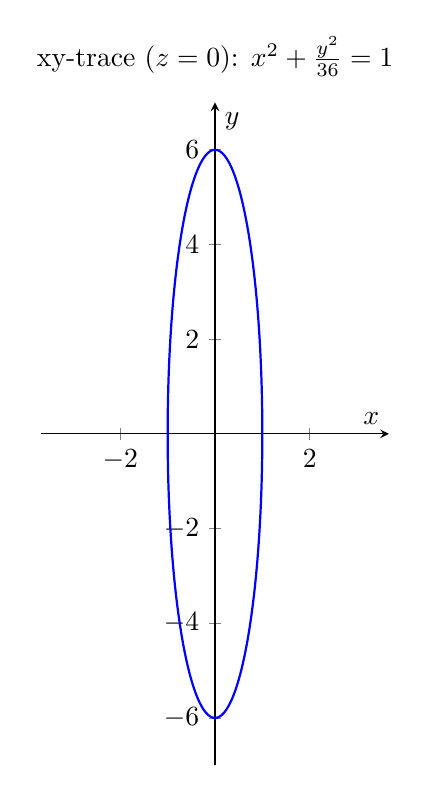
\begin{tikzpicture}
\begin{axis}[
    title={xy-trace ($z=0$): $x^2+\frac{y^2}{36}=1$},
    xlabel=$x$, ylabel=$y$,
    xmin=-2, xmax=2, ymin=-7, ymax=7,
    axis equal,
    width=6cm, height=10cm,
    axis lines=middle,
    samples=200
]
\addplot[blue, thick, domain=0:360] ({cos(x)},{6*sin(x)});
\end{axis}
\end{tikzpicture}
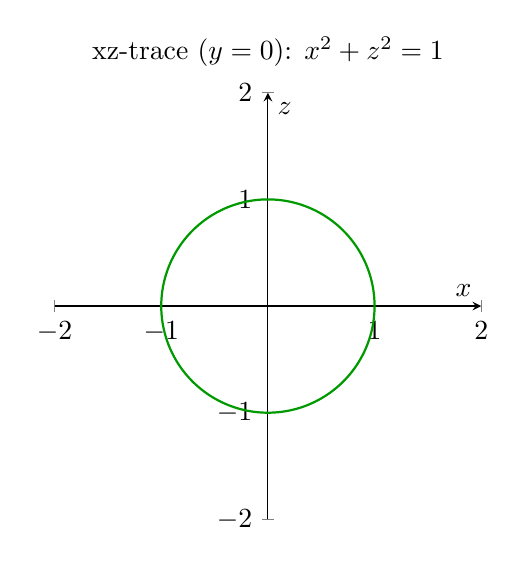
\begin{tikzpicture}
\begin{axis}[
    title={xz-trace ($y=0$): $x^2+z^2=1$},
    xlabel=$x$, ylabel=$z$,
    xmin=-2, xmax=2, ymin=-2, ymax=2,
    axis equal,
    width=7cm, height=7cm,
    axis lines=middle,
    samples=200
]
\addplot[green!60!black, thick, domain=0:360] ({cos(x)},{sin(x)});
\end{axis}
\end{tikzpicture}
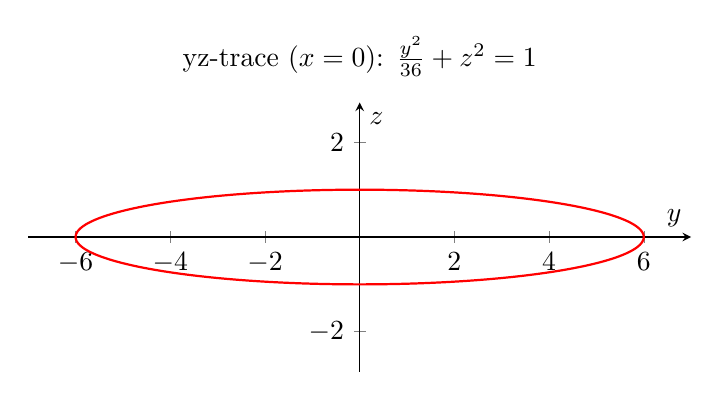
\begin{tikzpicture}
\begin{axis}[
    title={yz-trace ($x=0$): $\frac{y^2}{36}+z^2=1$},
    xlabel=$y$, ylabel=$z$,
    xmin=-7, xmax=7, ymin=-2, ymax=2,
    axis equal,
    width=10cm, height=5cm,
    axis lines=middle,
    samples=200
]
\addplot[red, thick, domain=0:360] ({6*sin(x)},{cos(x)});
\end{axis}
\end{tikzpicture}
\end{document}